\graphicspath{{figures/chapter4/}}

\chapter{Deep learning low-cost photogrammetry for 4D short-term glacier monitoring
  (2022-2023)}

\vfill

\newthought{This chapter is based on:}

\begin{itemize}
  \item Paper under review on PFG
  \item Ioli, F., Bruno, E., Calzolari, D., Galbiati, M., Mannocchi, A., Manzoni, P.,
        Martini, M., Bianchi, A., Cina, A., De Michele, C., and Pinto, L. (2023). A
        REPLICABLE
        OPEN-SOURCE MULTI-CAMERA SYSTEM FOR LOW-COST 4D GLACIER MONITORING, Int. Arch.
        Photogramm. Remote Sens. Spatial Inf. Sci., XLVIII-M-1-2023, 137–144, \\
        \url{https://doi.org/10.5194/isprs-archives-XLVIII-M-1-2023-137-2023}
\end{itemize}

\newpage

\section{Introduction}\label{sec:4:introduction}

{\color{red} TODO: write introduction}

\begin{figure}
  \centering
  \subcaptionbox{\label{fig:4:studyarea:map}}{
    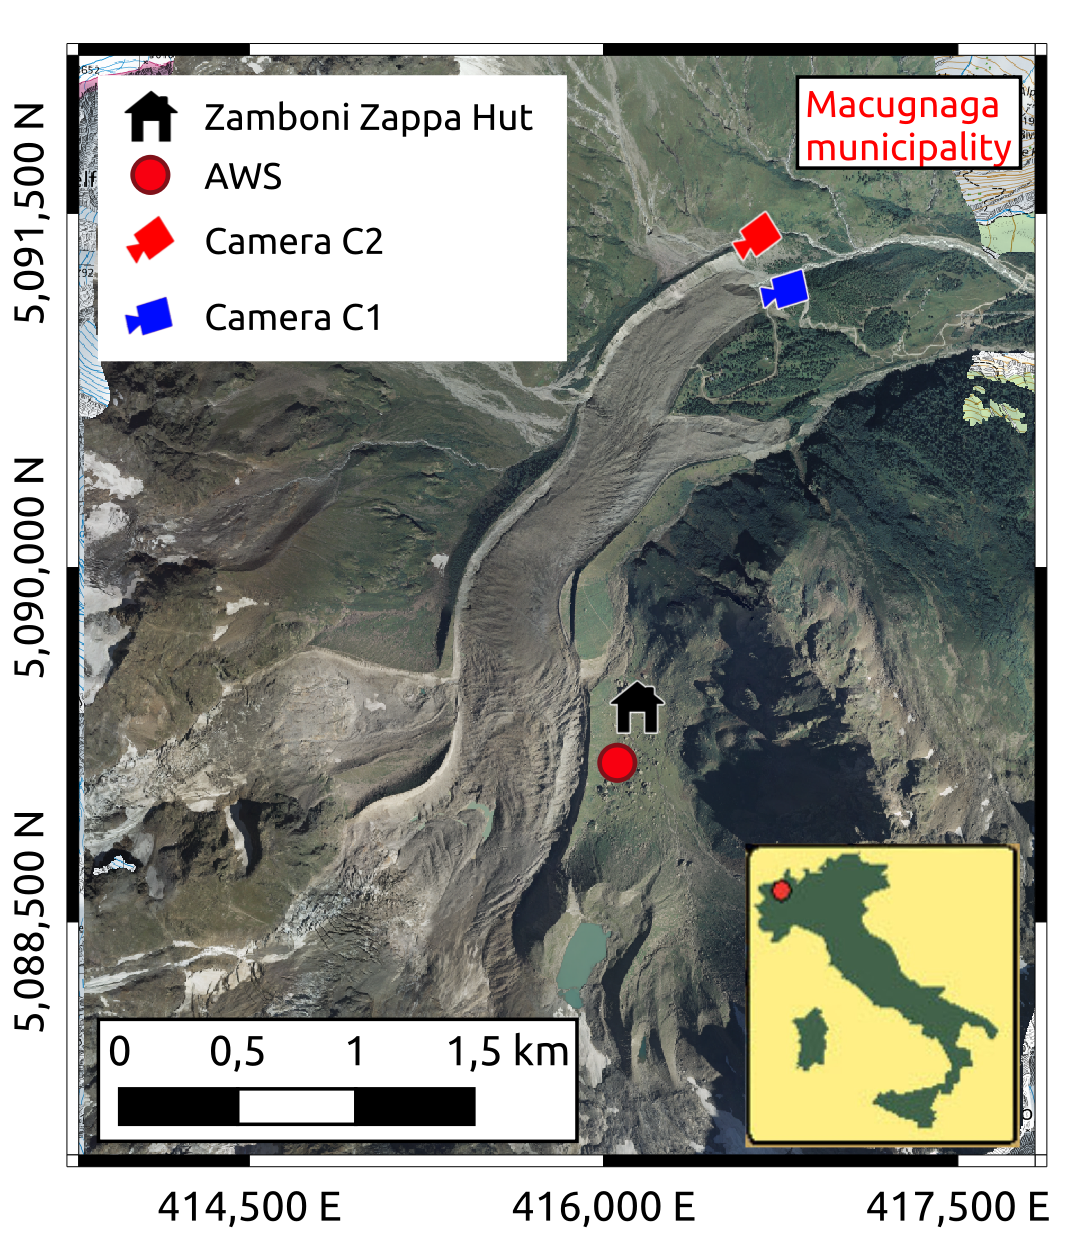
\includegraphics[width=.3\textwidth]{2_geographic_framework.png}
  }
  \subcaptionbox{\label{fig:4:studyarea:pic}}{
    \includegraphics[width=0.67\textwidth]{2_area_of_sudy.png}
  }
  \caption{(a) Map of the Belvedere Glacier, with marked the location of the two cameras
    C1 and C2, the Automatic Weather Station (AWS) and the Zamboni Zappa Hut;
    (b) The area of study: the stereoscopic reconstruction is focused on the terminal ice
    cliff (dashed light blue line), while the monoscopic DIC processing from camera C2
    image sequence is focused on the upper area of the north lobe (dashed green line).}
  \label{fig:4:studyarea}
\end{figure}

\section{The low-cost stereoscopic system}\label{sec:4:system}

% From last paper
The low-cost stereoscopic system consists of two autonomous and independent monitoring
units. Each unit is includes an off-the-shelf DSLR camera (Canon Eos 1200D), an Arduino
microcontroller for camera triggering, and a Raspberry Pi
Zero with a SIM card for sending images to a remote server via a GSM
network\citep{ioli2023_replicable}.
The instruments are housed in waterproof cases and mounted on tripods anchored to stable
rocks along the glacier moraines.
Power is supplied by a solar panel combined with a sealed lead-acid battery.
The total cost of each unit was less than \texteuro2000, including
camera and lens \citet{ioli2023_replicable}.
The low-cost camera system is described in detail in \citet{ioli2023_replicable}.

The two monitoring stations, labelled as C1 and C2, were installed in summer 2021 on
either side of the north tongue of Belvedere Glacier (\figref{fig:studyarea}).
The harsh glacier environment with steep and unstable moraines, often subject to rockfall
due to glacier retreat, constrained the camera installation location at
\SI{\sim230}{\meter} (camera C1) and \SI{\sim350}{\meter} (camera C2) from the terminal
ice cliff, with a strongly convergent pose.
Different lenses were used for the two cameras to achieve the same image scale in
correspondence of the glacier tongue: C1 was equipped with a 24 mm lens, while a 35 mm
lens was used for C2.

\begin{table}
  \centering
  \caption{Summary of the characteristics of the two cameras.
    Fields marked with $^*$ are computed considering the distance between each camera and
    the ice cliff.}
  \label{tab:cameras}
  \begin{tabular}{c c c}
    {}              & C1                               & C2 \\
    \hline\noalign{\smallskip}
    Camera          & Canon Eos 1200D
                    & Canon Eos 1200D                       \\
    Sensor          & APS-C
                    & APS-C                                 \\
    Pixel size      & \SI{3.7}{\micro\meter}
                    & \SI{3.7}{\micro\meter}                \\
    Image           & \qtyproduct{6000x4000}{\pixel}
                    & \qtyproduct{6000x4000}{\pixel}        \\
    Lens            & Canon EF 24mm f/2.8 IS USM
                    & Canon EF 35mm f/2 IS USM              \\
    Distance$^*$    & \SI{230}{\meter}
                    & \SI{350}{\meter}                      \\
    Average GSD$^*$ & \SI{3.5}{\centi\meter\per\pixel}
                    & \SI{3.5}{\centi\meter\per\pixel}      \\
    \noalign{\smallskip}\hline
  \end{tabular}
\end{table}

The baseline between the two cameras of \SI{\sim 261}{\meter} ensured a good
viewing geometry because of the large parallax between corresponding points.
However, the baseline comparable to the camera-object distance (base-height ratio close
to \(1\), \tabref{tab:cameras}) led to complex affinity-like distortions and occlusions
between corresponding areas in the two images~\citep{Yao_2021}.
Additionally, C1 was positioned at a lower viewpoint compared to C2, due to
site geometry constraints.
Therefore, camera C1 provides a limited view that primarily encompasses the frontal ice
cliff, but does not capture the glacier surface, which is only visible from camera C2.

The stereoscopic system was operating from August 2021 up to December 2022, when it was
temporarily unmounted for ordinary maintenance, and finally mounted again in June 2023.
During the operational period, the system was programmed to acquire two images per day,
but only one image per day was used for the multitemporal processing.
Only daily images taken during the snow-free period between 01/05/2022 and
13/11/2022 were considered.
In this period, the glacier is experiencing the most significant changes, flow velocity
and ablation rates. On the other hand, during winter and spring seasons, the glacier was
covered by snow, making it difficult to extract relevant information from optical images
for tasks such as 3D reconstruction and surface velocity estimation.

% From paper antalya
The low-cost stereoscopic system for continuous monitoring is composed of two independent
units, each housing an off-the-shelves DSLR camera.
Each unit consists in an autonomous monitoring station that provides power supply,
internet connectivity, timing and scheduling of image acquisition, and protection from
the harsh environment.
The station was designed and built adapting to the alpine environment an existing
open-source model developed by Greig Sheridan and published on
GitHub\footnote{\label{foot:greig}Greig Sheridan' Intervalometerator repository:
  \url{https://github.com/greiginsydney/Intervalometerator}}.
A key aspect of the project was to ensure easy assembly and realization of the system to
guarantee future replication or improvement by non-experts.
In the following, we describe in detail the services and the
nominal performances provided by our system that make it worth consideration for
applications in different monitoring contexts. Refer to \figref{fig:scheme_foto} for
a descriptive schematic of the whole system showing the components selected for the
Belvedere Glacier case study. The choice of the camera and optics is discussed in Section
XX, as these components are dependent on the domain of use of the
stereoscopic system.

\begin{figure}[h!]
  \centering
  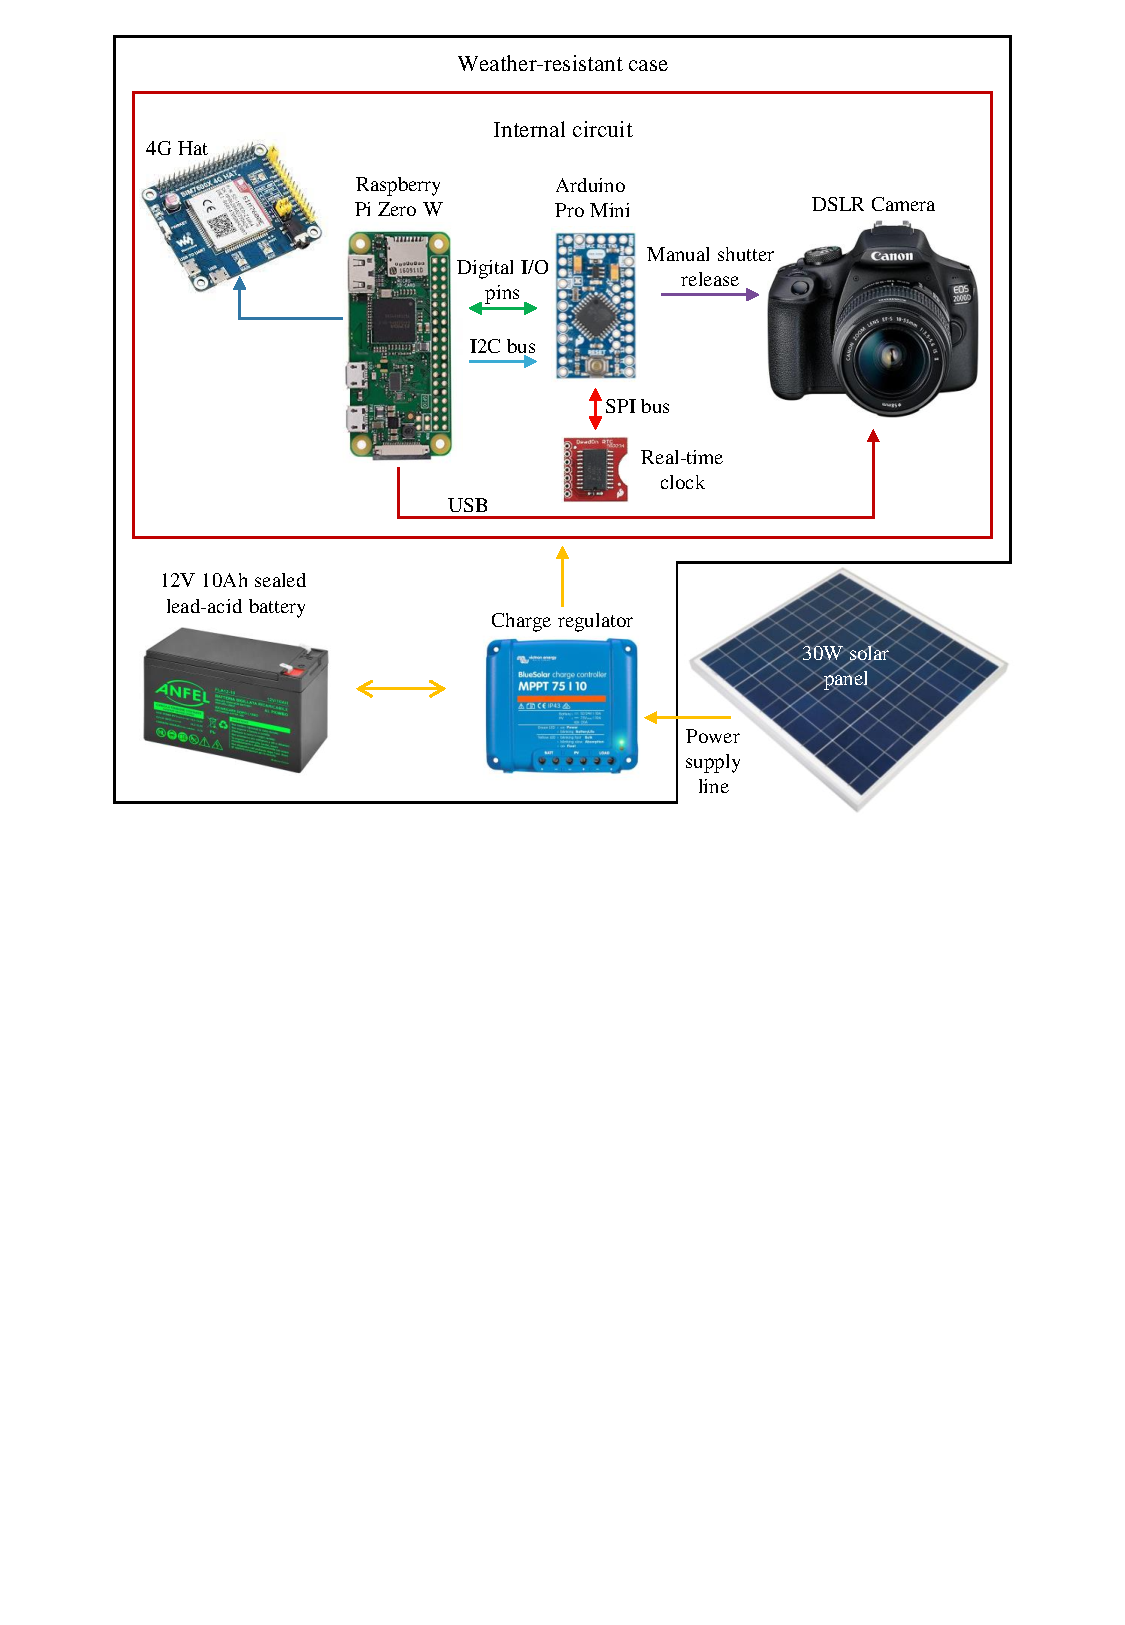
\includegraphics[width=0.6\textwidth]{schema.pdf}
  \caption{Scheme of the proposed acquisition system configuration for a single
    monitoring station. Arrows indicate the direction of signal initiation. Image adapted
    from Greig Sheridan's repository.}
  \label{fig:scheme_foto}
\end{figure}

\subsection{Power supply}\label{Power_supply}
Each monitoring unit has its autonomous power supply line (yellow arrows in Figure
\ref{fig:scheme_foto}) provided by a solar panel combined with a sealed lead-acid
battery. An MPPT (Maximum Power Point Tracker) charge regulator directly connects with
the unit's internal circuit, providing a regular current supply to the battery
and the load and exploiting all the power generated by the panel. This regulator prevents
any excess current that may damage the connected device, thus increasing the reliability
of the system. Its battery life-saving algorithm modulates the load disconnection level
so that a nearly 100\% recharge is achieved about once every week and, in case of battery
discharging, the whole system is switched off until 100\% recharge of the battery is
achieved.
The whole monitoring system is designed to minimise power consumption, e.g., by powering
off devices responsible for the highest power consumption when not needed.
An estimation of the system's energy consumption guided the choice of the components of
the power supply line. Specifically, the battery and the associated panel must be
accurately dimensioned for the system's purpose. To this end, the Photovoltaic
Geographical Information System (PVGIS) \citep{pvgis}, a tool provided by the European
Commission, was used. PVGIS can estimate the performance of off-grid photovoltaic systems
according to the installation site and it is supported by a database and algorithms for
calculating solar radiation. Tuning the parameters for the Belvedere Glacier location and
the system consumption, we ended up with the specifications of solar panel power of 30 W
and battery voltage of 12 V and capacity of 10 Ah. Some compromises were made, accepting
that the system would not be sufficiently powered in the months with lowest solar
radiation (November, December, January, and February). {\color{red} further details on
    PVGIS simulations for the Belvedere Glacier case study re given.}

\subsection{System control and scheduling}\label{Control}

\begin{figure}[ht!]
  \centering
  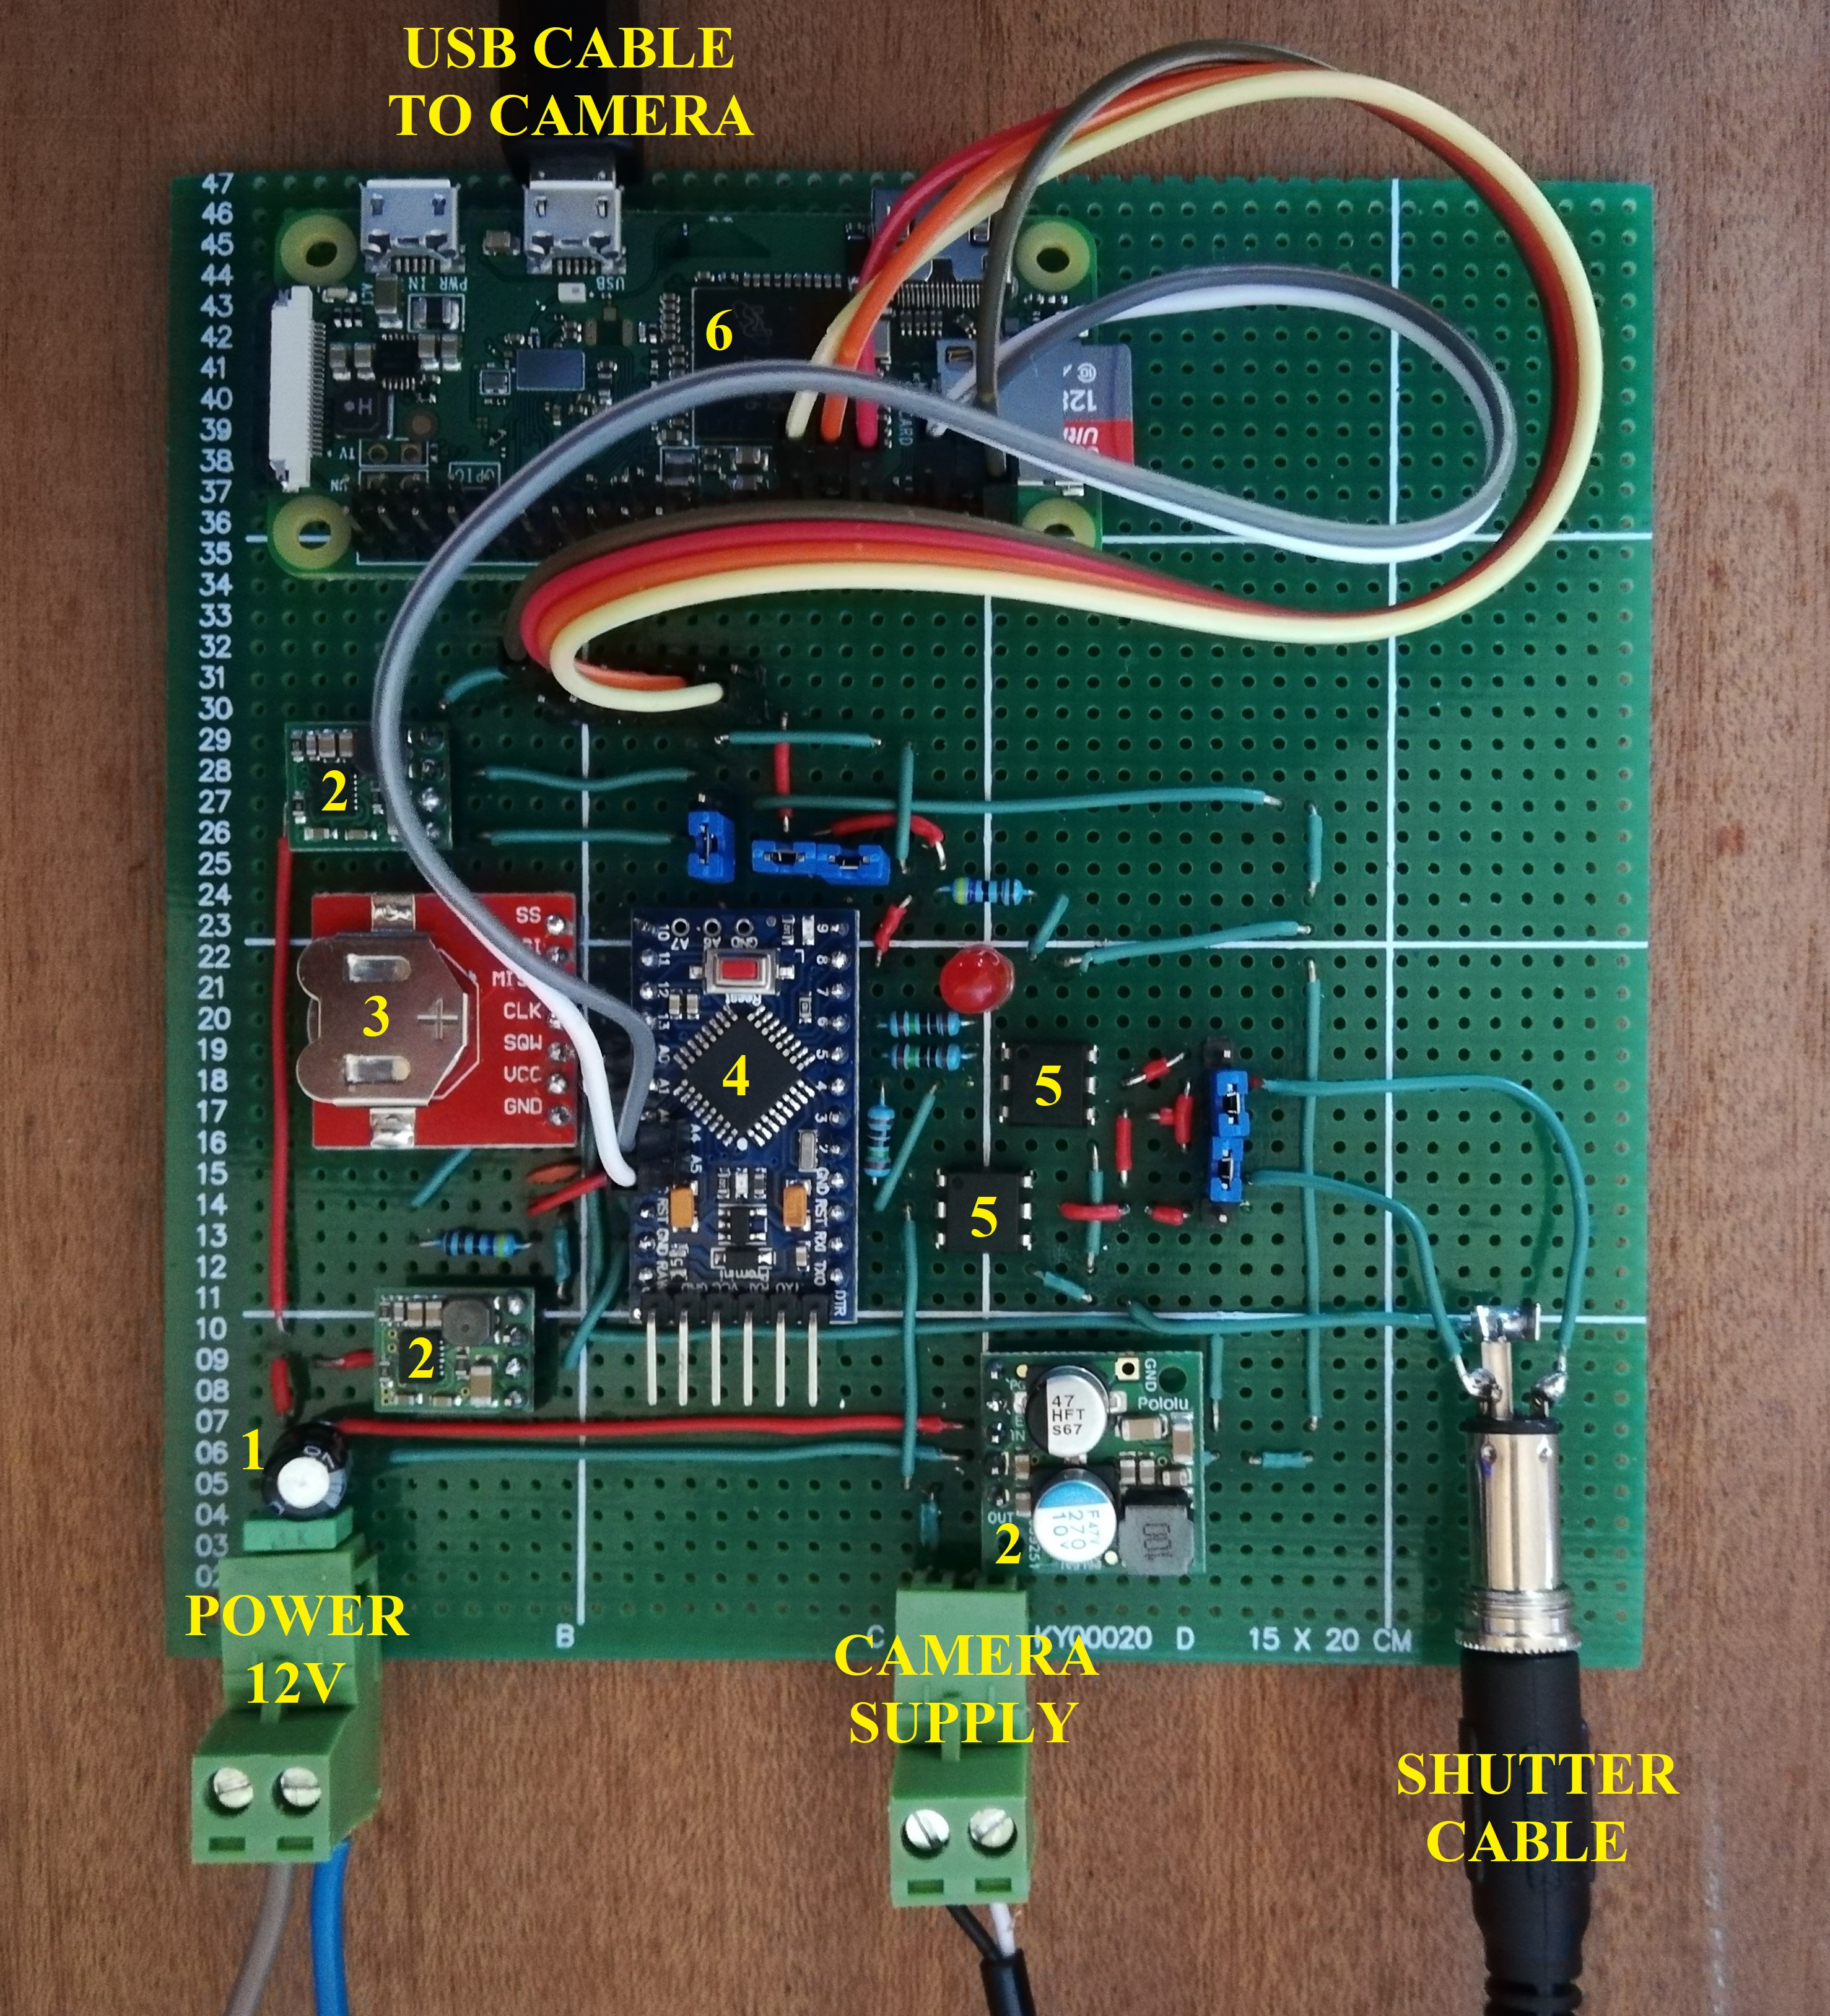
\includegraphics[width=0.6\textwidth]{board.jpg}
  \caption{Stripboard on which are soldered the main components of the internal
    circuit: capacitors (1), voltage regulators (2), real-time clock with coin-cell
    battery
    (3), Arduino Pro Mini (4), optoisolators (5), and Raspberry Pi Zero W (6).}
  \label{fig:circuit}
\end{figure}

The internal electronic circuit (red box in Figure \ref{fig:scheme_foto}) of the
monitoring unit is the only load connected to the power supply and is responsible for all
the system's control and scheduling functionalities.
Its components are a real-time clock (number 3 in Figure \ref{fig:circuit}) with a 12 mm
coin-cell backup battery, an Arduino microcontroller (Pro  Mini 328 3.3V 8MHz, number 4
in Figure \ref{fig:circuit}), a Raspberry Pi Zero W with 128 GB SD memory card (number 6
in Figure \ref{fig:circuit}), and minor elements for connections, isolation (capacitors
and optoisolators numbers 1 and 5 in Figure \ref{fig:circuit}), and voltage regulations
(numbers 2 in Figure \ref{fig:circuit}).
The circuit was realized manually by soldering wires and components on a stripboard (see
Figure \ref{fig:circuit}).

The Arduino communicates through an SPI (Serial Peripheral Interface) bus with an
accurate real-time clock to schedule its actions: waking the camera, firing the shutter
to take a photo, and turning on/off the Raspberry. The Raspberry is able to access the
camera images and transfer them to a remote server via internet connectivity. A large
storage memory is added to the unit to save photos before remote transferring. The
Raspberry also provides a web-based, user-friendly interface (Figure
\ref{fig:web-interface}) to configure and monitor the system remotely \citep{greig}. An
I2C (Inter Integrated Circuit) bus and digital pin connections enable higher-level
communication between these two boards. Among the minor components, we mention the role
of the three voltage regulators. They allow each unit to be powered at the appropriate
voltage and current: starting from the 12 V in input, one delivers 3.3 V and 500 mA to
the Arduino, one 5 V and 2.5 A to the Raspberry and its hat, and the other 7.5 V and 2.4
A to the camera. The Arduino controls the 5V regulator of the Raspberry to reduce
quiescent power consumption when the Raspberry board is off.

Acquisition of a defined number of images, camera triggering and timing, and sending of
images to a remote server can be scheduled thanks to adequate programming of a cyclic
executive program in C++ for Arduino and  of services executing automatically Python
scripts for the Raspberry.
All the monitoring station activities can be remotely scheduled from the terminal or a
user-friendly web interface \citep{greig}. This useful feature allows one to change the
settings and check the behaviour of the system, avoiding the need for manual
intervention. The Raspberry uses the gPhoto2, a Python-based protocol developed to
specifically interact with popular cameras’ firmware, to communicate with the camera and
access the new photos. The  web-based interface service is based on NGINX and Gunicorn,
open-source software for web servers. The interface (Figure~\ref{fig:web-interface})
consists of a web page accessible with credentials and provides a summary of the system
state and the exact time of the last operations (time of the last shot and the last
upload of images), temperatures of the components, previews of the last images, buttons
to wake up the camera, take a preview photo and schedule the system routine (time and
number of photo acquisition, wake-up time of the Raspberry) and some camera settings.

\begin{figure}[h!]
  \centering
  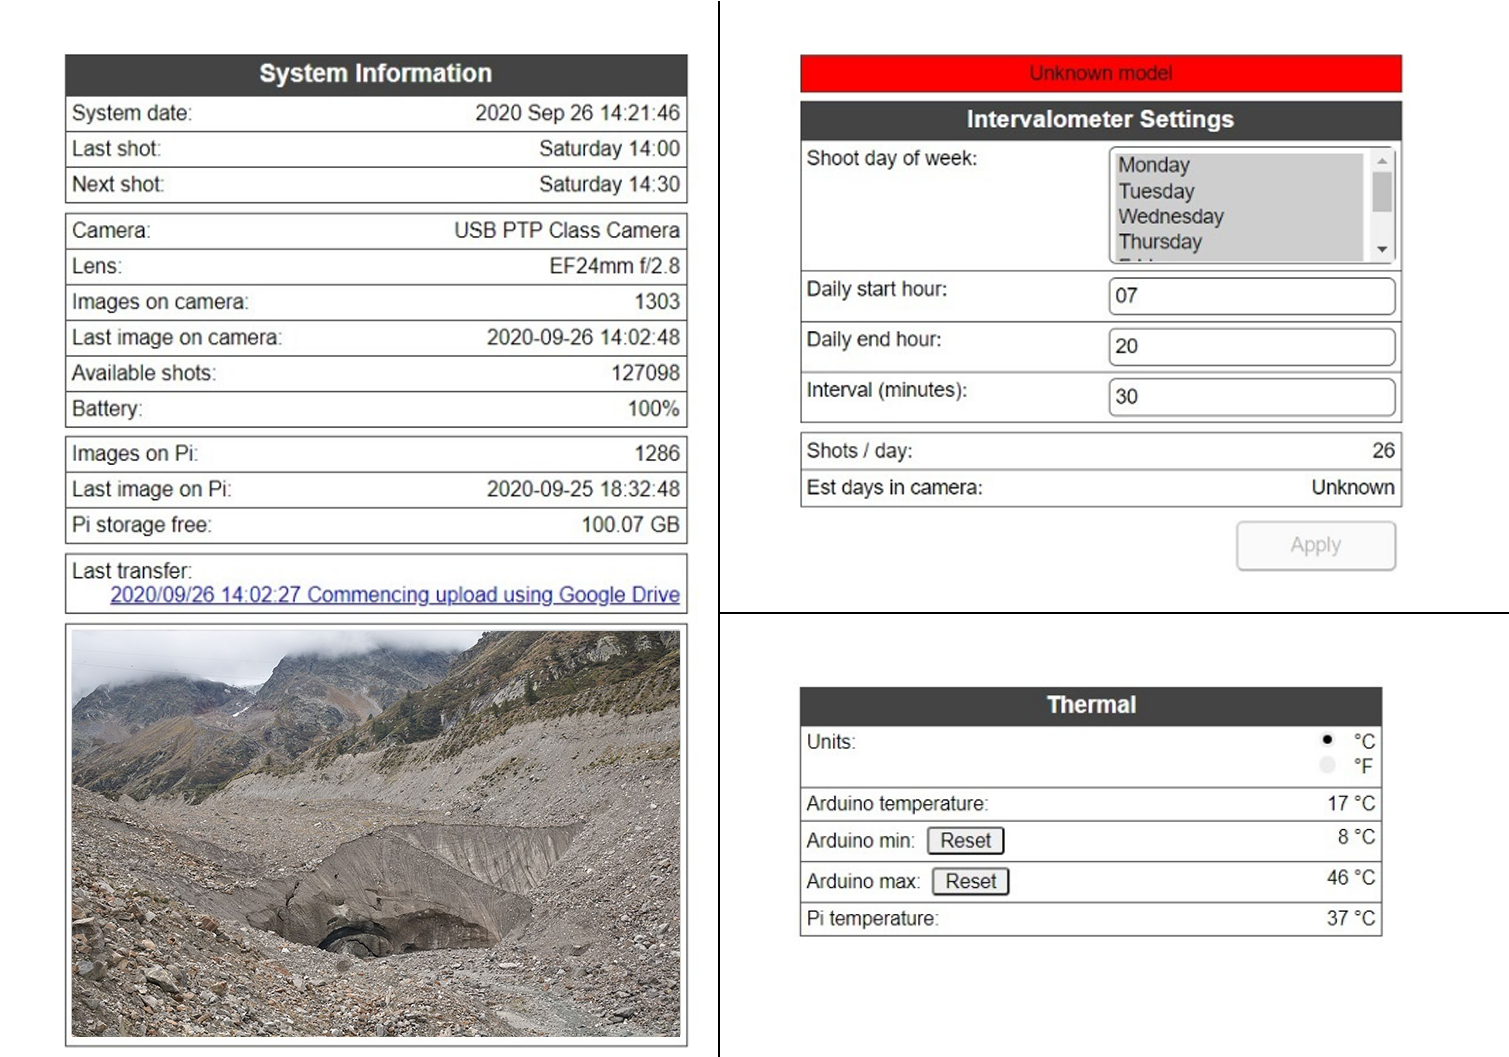
\includegraphics[width=0.8\textwidth]{web_interface.png}
  \caption{Example of some of the pages of the web-based interface to remotely control
    the monitoring units.}
  \label{fig:web-interface}
\end{figure}

All the components were chosen because of their low power consumption and their
inter-compatibility. The circuit is robust against power losses due to battery
discharging and is able to auto-recover when power is regained. A low energy consumption
policy is also followed in selecting the scheduling. The camera is switched on only
during the data capture activity. The Raspberry is switched on only once per day when the
connection with the remote server and image transfer is scheduled.

\subsection{Connectivity}\label{Connectivity}
Internet connectivity is crucial to transfer images and to control the units remotely. To
this end, the Raspberry is equipped with the SIM7600E-H 4G hat by Waveshare. The module
supports 4G/3G/2G communication via a SIM card. Raspberry and hat operations are the most
expensive in terms of power consumption. For this reason, the board is switched on only
once a day for a limited period of time, which is kept adequately low to be sustainable
for the system power supply but still sufficient for transferring new images to the
server. We adopted IoT (Internet of Things) SIM cards provided by the multi-operator
service Emnify \citep{emnify}, as it offers the ability to connect to the best-quality
cellular network available and includes flexible and customizable data plans.
Remote access to the devices is allowed by a VPN (Virtual Private Network).
The service costs \texteuro33 per month for a data plan with 6 GB.

\subsection{Case and protection}\label{Case and protection}
The majority of the components need to be protected. Therefore, a solid and compact case
that allows keeping all the parts (with the exception of the solar panel) in the same
location is desirable for the functioning of the system and for convenient
transportation, installation and maintenance. The case should also satisfy the thermal
insulation requirements according to each component's working temperature range. The case
should also be waterproof and robust against different and harsh weather conditions but,
at the same time, provide access for connecting the solar panel and taking pictures. Our
choice was an HPRC 2250 lightweight, waterproof resin case with internal insulating foam.
The foam was found to be useful in enhancing the temperature seal and stabilising the
location of some components, preventing unwanted movements. Holes were drilled in the
case: one sealed with a UV filter of 82 mm to allow the camera to take shots, two others
to give access to the solar panel wires, and others to fix the system to a tripod. The
internal case dimensions (236x182x155 mm) posed a significant challenge in accommodating
all the components inside. In particular, the camera lens dimensions were constrained by
space availability.

\subsection{General performances}\label{General_performances}
The system was subject to several tests before being used in its final application at the
Belvedere glacier site. During these tests, the system proved to be autonomous, robust to
sudden shutdowns, cold-resistant, water-resistant and self-sufficient for a prolonged
period of time with no direct sunlight on the solar panels. Specifically, in the absence
of sunlight, the battery is able to power the system for about nine days before it is
completely discharged. Battery voltage and temperatures of components were monitored,
simulating the absence of solar radiation and low environmental temperatures. See Figure
\ref{fig:nominal} for the performances of the system during these tests.
\begin{figure}[h!]
  \centering
  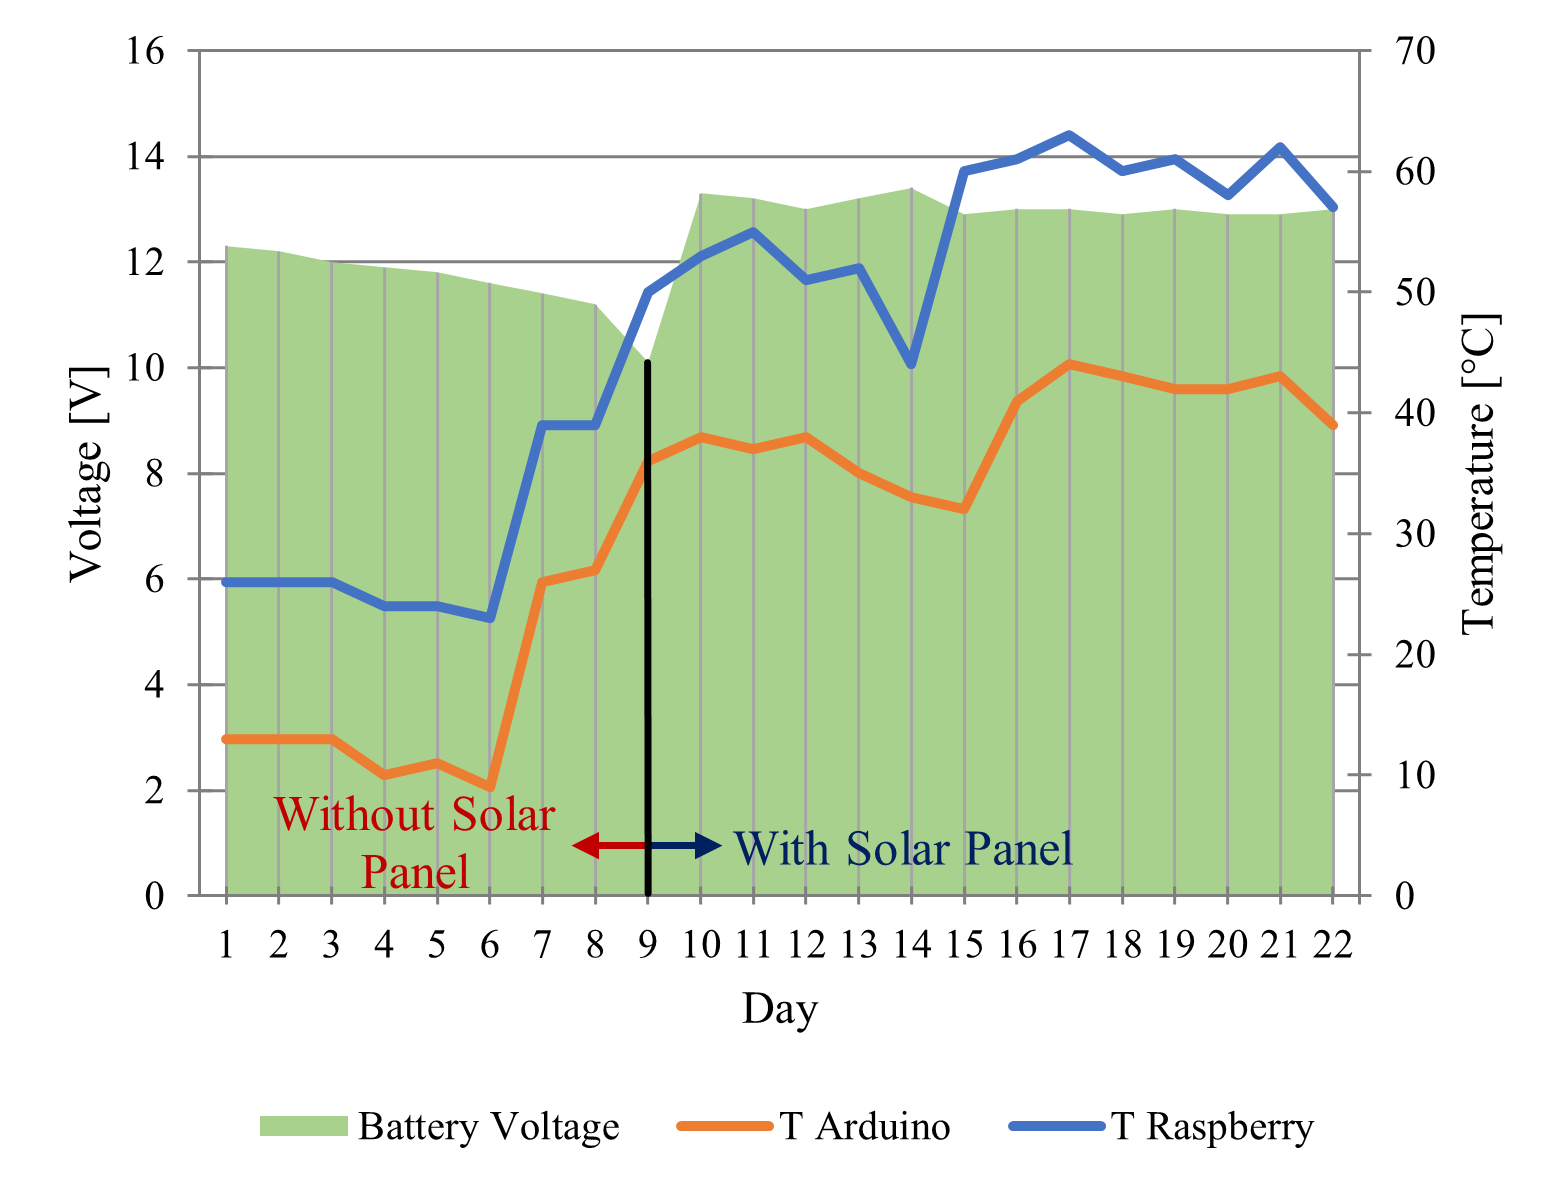
\includegraphics[width=.5\textwidth]{nominal.png}
  \caption{Battery voltage and temperature of boards with and without the solar panel
    during a period of tests. Starting from a fully charged condition, the system was
    kept
    without solar panel at around 2 °C for the first six days. After nine days, the
    battery
    was fully discharged and the system was reconnected to the panel and exposed to solar
    radiation.}
  \label{fig:nominal}
\end{figure}

\subsection{Camera and lenses}\label{camera_lenses}
The choice of the DSLR camera and of the optics can be considered application-dependent.
Therefore specifications regarding these components are reported in reference to the
Belvedere glacier case study. Each monitoring station was equipped with a DSLR camera
Canon EOS 2000D, with 24.1 MP CMOS \mbox{APS-C} sensor. This model was chosen because of
the limited costs, the high image resolution and its compactness, as it must fit inside
the case. Additionally, another fundamental requirement was camera compatibility with the
gPhoto2 software. In the installation inside the system case, the traditional
rechargeable battery was replaced by a special battery (”fake battery”) equipped with a
power supply cable, which provides a voltage of 7.5 V from the circuit. The camera is
attached to a sliding plate able to vary, with a limited range, and then fix the position
of the camera on the longitudinal axis. Screws fix the camera to the plate and the plate
to the case.

The two stations were installed respectively at $\sim$180 m and $\sim$340 m distance to
the glacier terminus (see Figure \ref{fig:4:studyarea}), avoiding the steep moraines
of the glacier, often prone to collapses and landslides. Therefore, a wide baseline of
$\sim$260 m occurs between the two sensors.
The final positioning of the two cameras was decisive in the choice of optics.
In fact, to ensure comparable Ground Sample Distance (GSD) of the images ($\sim$3 cm
px$^{-1}$), lenses with different focal lengths were employed.
In particular, a Canon EF 24 mm f/2.8 IS USM and a Canon EF 35 mm f/2 IS USM were used
respectively for Camera 1 (stream-wise right) and Camera 2 (stream-wise left).

\subsection{Camera installation}\label{Monumentation}

Monumentation of the two cameras at the Belvedere Glacier site was achieved by choosing
two large stable rocks along the moraines.
Each camera is supported by an aluminium topographic tripod system anchored with steel
dowels and cables to the rocks (Figure~\ref{fig:final_installation}b).
A central steel tie rod keeps the system in a fixed position.
The choice of an agile monumentation was aimed at having a system that can be rather
easily assembled on site (and also disassembled, if needed), also in a harsh environment,
with limited costs and time.
To install the cameras, in fact, all the equipment was carried in backpacks along the
moraines, sometimes without a marked walking path (e.g., in the case of the stream-wise
left camera).
As a drawback, the analysis of the acquired photos revealed a non-optimal stabilization
of the two cameras.
In fact, small rotations, especially around the vertical axis, and vibrations, mostly
induced by the wind, were experienced.
Though, a perfectly stable monumentation in a mountain environment is hardly achievable.
Therefore, it is not possible to assume the camera orientation as stable a priori, but
camera orientation must be estimated based on some Ground Control Points (GCPs) located
on the ground in stable areas.

It is worth mentioning the performances of the system in terms of costs: our  monitoring
system can be fully reproduced with an average cost of \texteuro2000 per station
(November 2023), including camera (\texteuro400), lens (\texteuro500) and material for
the on-site installation (\texteuro150).
In comparison, commercial time-lapse cameras are expensive
(e.g., PhotoSentinel\footnote{PhotoSentinel: \url{https://photosentinel.com/} (accessed
  on 15/11/23)} cameras cost more than \$5,000.00) and hardly customizable.
The final prototype of the monitoring station is shown in Figure
\ref{fig:final_installation}.

\begin{figure}[h!]
  \centering
  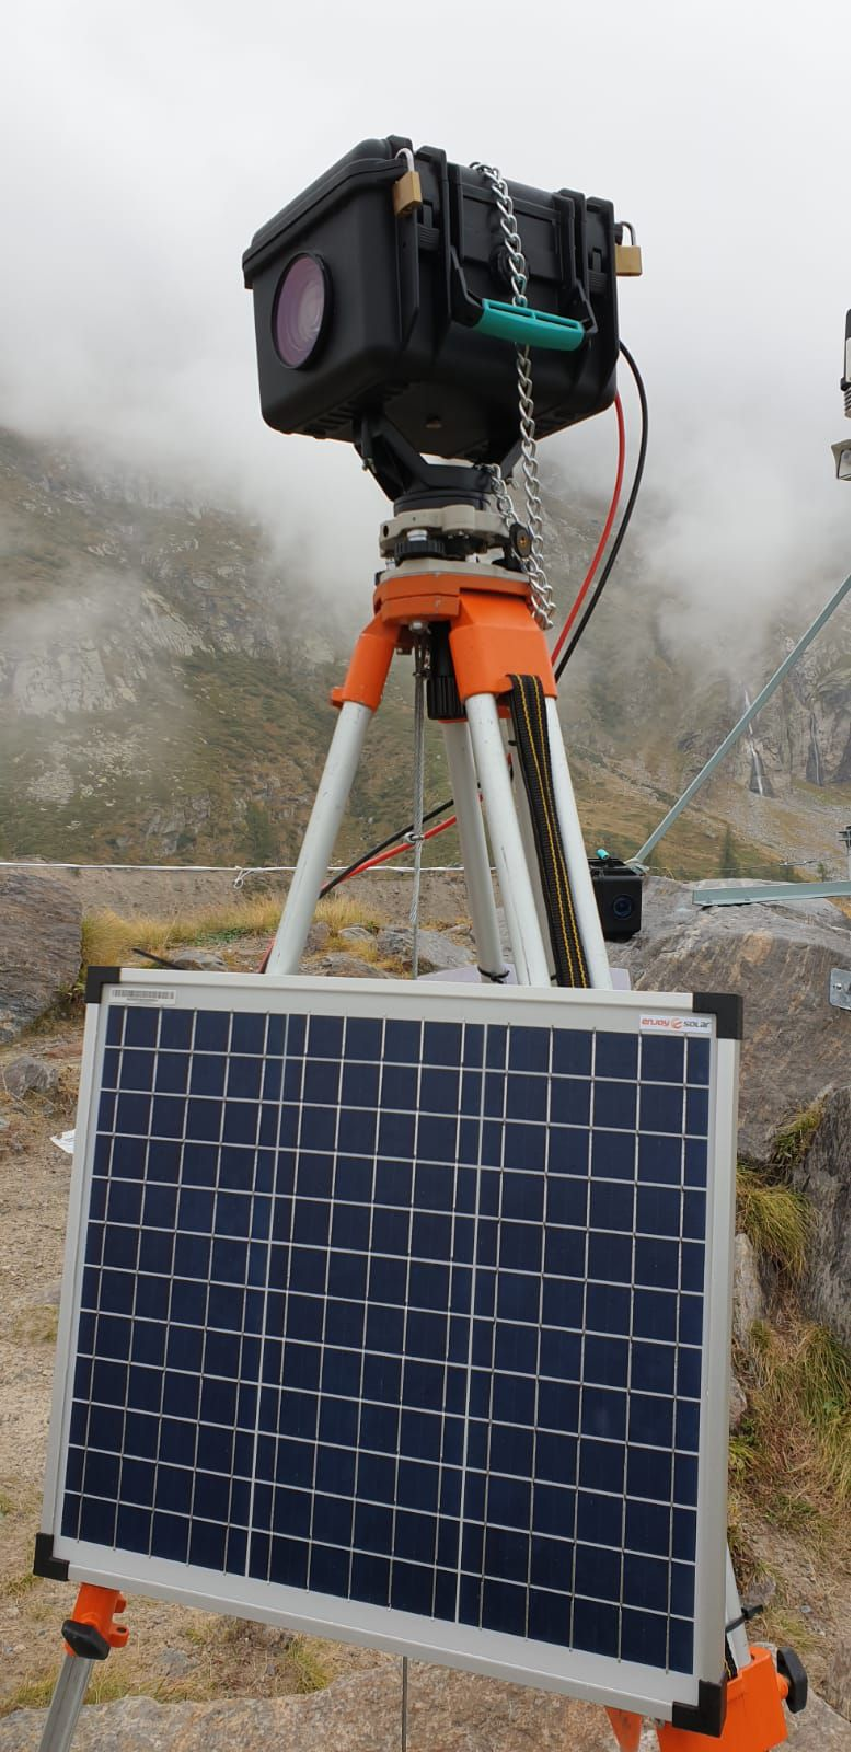
\includegraphics[width=.2\columnwidth]{finale1.pdf}
  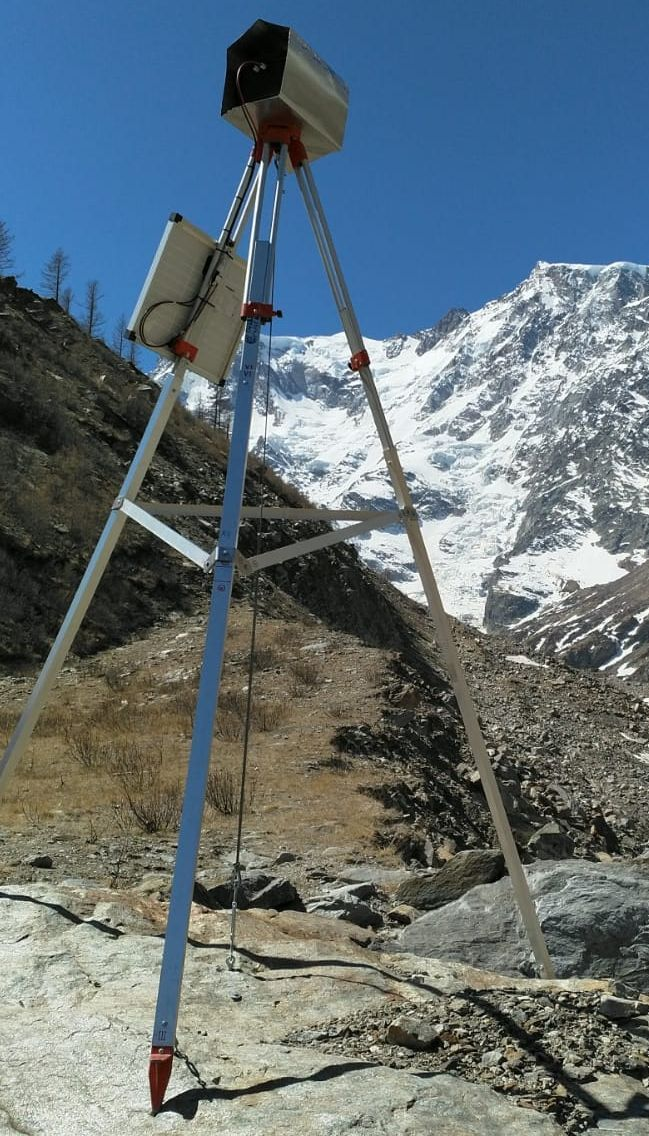
\includegraphics[width=0.3\columnwidth]{centralina.jpg} \\
  \centering{(a)\hspace{30mm}(b)}\\ \vspace{1mm}
  \caption{(a) Picture of the monitoring unit prototype installed for tests at the
    Belvedere Glacier site. (b) Picture of the final monumentation of the camera
    installed on
    the stream-wise right moraine. {\color{red} TODO: change picture with the final
        installation}}
  \label{fig:final_installation}
\end{figure}

\section{Datasets}\label{sec:4:datasets}

\subsection{stereoscopic image sequences}\label{sec:4:stereo}

During the snow-free study period (from 1/05/2022 to 13/11/2022), both camera C1 and
camera C2 were able to acquire images every day, for a total of 197 images. However, 39
images were discarded due to bad weather conditions, such as rain, low clouds, or fog,
resulting in 158 days with valid data for stereo and monoscopic processing

  {\color{red} TODO: write about the images sequence 2022 and 2023}

\subsection{UAV surveys}\label{sec:uavsurveys}

Two UAV flights, spaced by a 10-days interval, were conducted in summer 2022 to acquire
ground truth data for assessing the proposed methodology.
The first UAV flight, labelled as UAV-A, was carried out on 28/07/2022 with a DJI
Matrice 300 RTK quadcopter and a DJI Zenmuse P1 camera with a 35 mm lens.
During the survey, 436 images were captured, encompassing both nadiral and oblique
perspectives.
Additionally, 19 Ground Control Points (GCPs) were measured using a combination of a
total station and Differential GPS (DGPS), employing a topographic-grade
GNSS receiver.
The GCPs included both artificial targets and natural features.
During the flight, the UAV was equipped with an on-board RTK GNSS receiver, enabling the
acquisition of camera projection centers with decimetric accuracy.
The photogrammetric block (\figref{fig:uavblocks}a) was processed with the commercial
software package Agisoft Metashape \citep{agisoft} by using 14 GCPs and 5 Check Points
(CPs) to evaluate the block accuracy.
The global RMSE evaluated on the CPs was equal to 4.0 cm.

The secondo UAV flight, UAV-B, was carried out on 05/08/2022 with a DJI Phantom
4 RTK, focusing on a smaller portion of the northern lobe of the Belvedere Glacier.
However, due to technical constraints, \textit{moving} GCPs located inside the
glacier body were not measured again.
Therefore, only the fixed targets located outside the glacier were employed.
Among these, 8 targets were designated as GCPs, while the remaining 4 were used as CPs.
The photogrammetric block encompassed 428 nadiral and oblique images, which
were processed using Agisoft Metashape (\figref{fig:uavblocks}b).
A global RMSE of 7.5 cm was obtained on the 4 CPs.

\begin{figure}
  \begin{center}
    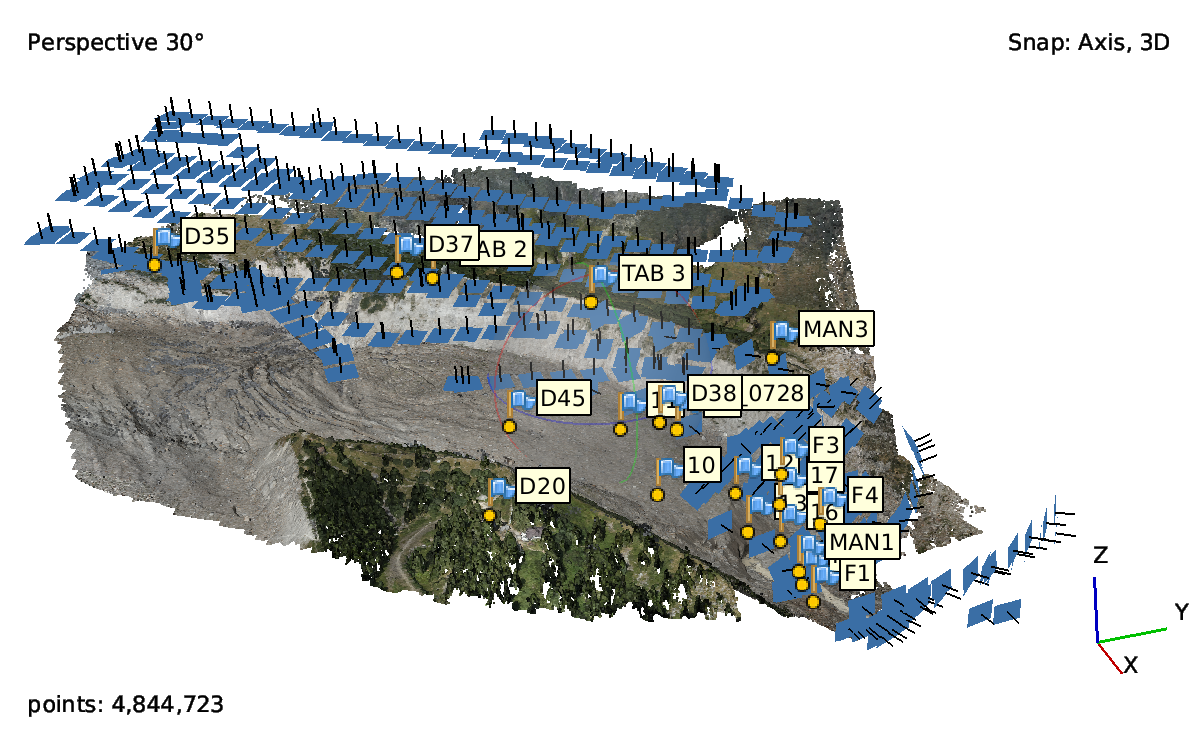
\includegraphics[width=84mm]{2_UAV-A_280722.png}
    \centering{(a)} \\ \vspace{1mm}
    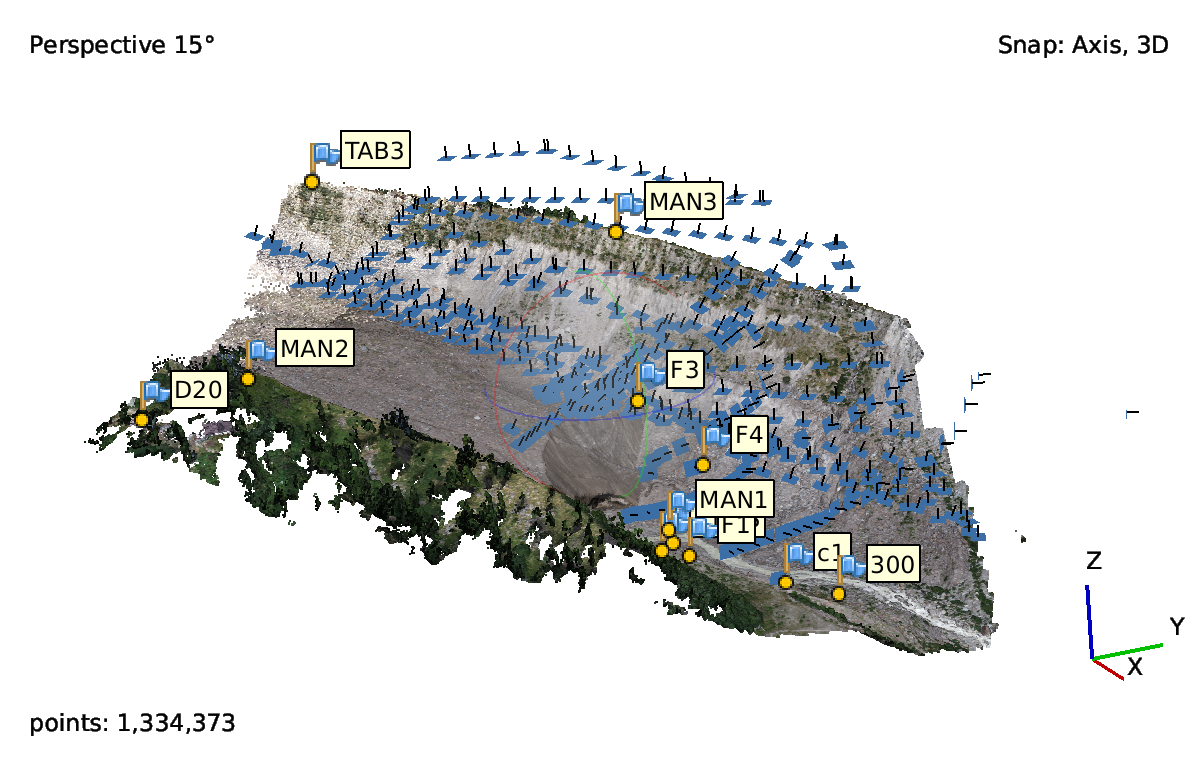
\includegraphics[width=84mm]{2_UAV-B_050822.png}
    \centering{(b)}
  \end{center}
  \caption{(a) UAV-A block and (b) UAV-B block processed with Agisoft Metashape. The
    flags represent the targets used either as GCPs in the BA or as CPs to evaluate the
    quality of the photogrammetric block.}
  \label{fig:uavblocks}
\end{figure}

\subsection{Meteorological monitoring station}\label{sec:meteostation}

To analyze the correlation between the Belvedere Glacier dynamics and
external environmental variables, data measured from an Automatic Weather Station (AWS)
located close to the Zamboni Zappa Hut were used.
The AWS is located at an altitude of \SI{2075}{\masl} and at a distance of
2 km from the area of study.
In our study, we analyzed mean daily values of air temperature, precipitation and
incoming solar radiation from 01/05/22 to 15/11/22.

\section{Methodology}\label{sec:methodology}
This chapter outlines the methodology developed to monitor the evolution of the Belvedere
Glacier northern lobe.
The daily images were processed using a framework consisting of two parallel processing
chains (\figref{fig:workflow}):
(i) a photogrammetric-based stereoscopic approach;
(ii) a DIC-based monoscopic approach.
The daily stereo pairs were used to generate 3D models of the glacier terminus,
enabling the estimation of ice volume loss on a daily basis by computing point cloud
differences along the main flow direction.
However, due to limited overlapping views of the two cameras, the stereoscopic approach
primarily provides a 3D reconstruction of the terminal ice cliff (dashed-blue area in
\figref{fig:studyarea}b).
Consequently, deriving the 3D surface velocity field of the glacier solely from
photogrammetry was not feasible.
The image sequence captured by camera C2, offering a higher viewpoint and broader
coverage of the glacier surface, was employed to determine the glacier's surface velocity
over a larger area of the north lobe of the Belvedere Glacier (dashed-green area in
\figref{fig:studyarea}b).

\begin{figure*}[ht]
  \centering
  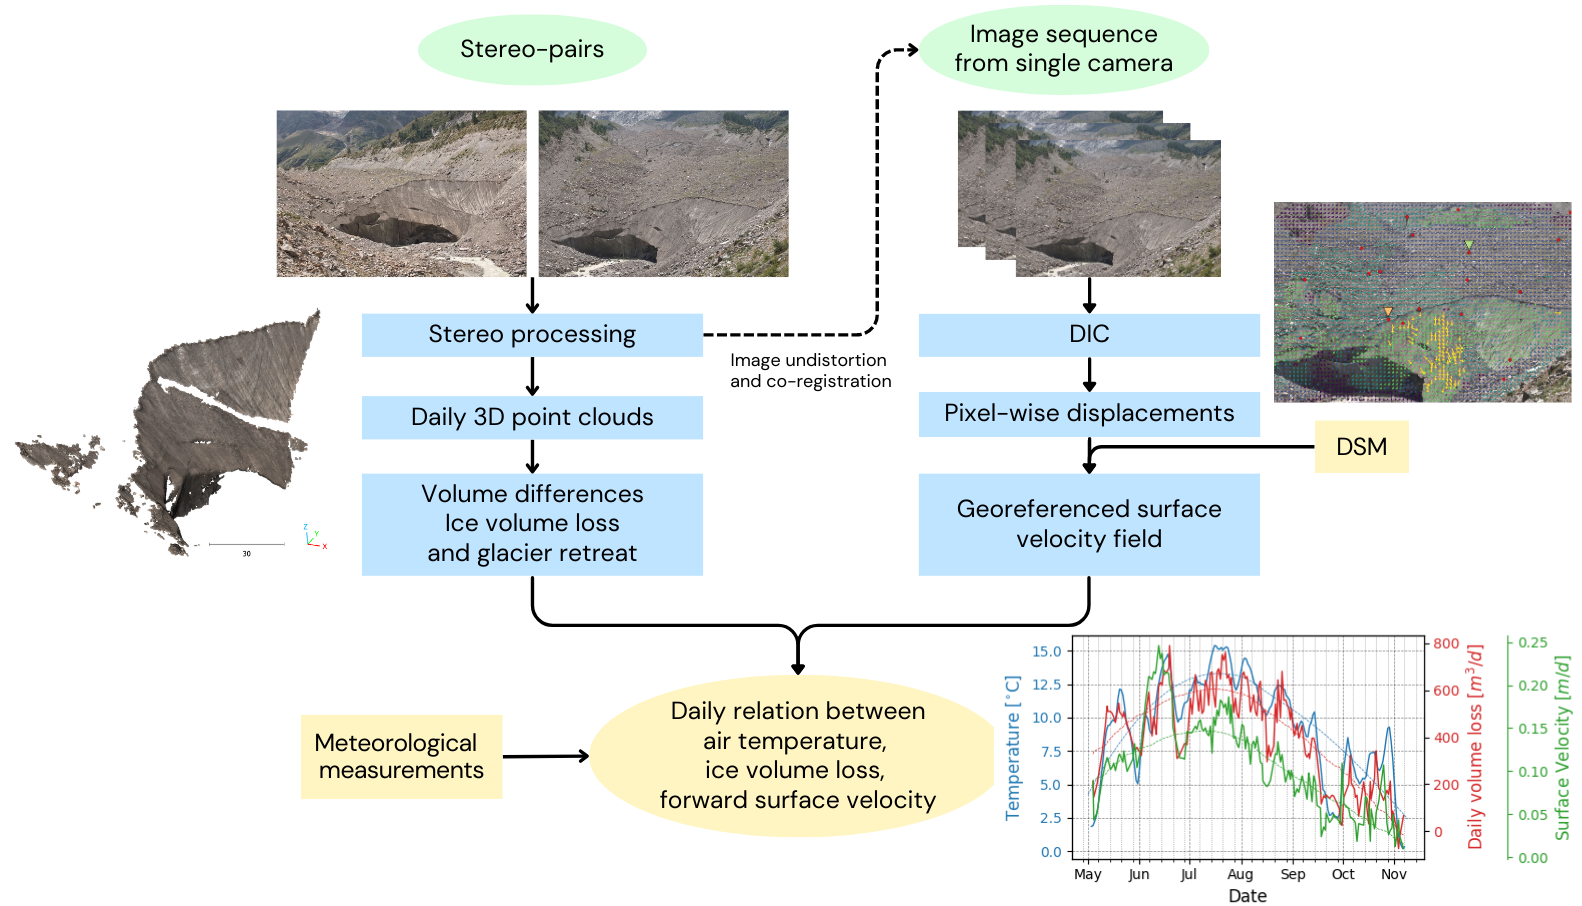
\includegraphics[width=154mm]{3_general_workflow.png}
  \caption{General workflow with two parallel processing chains involving stereoscopic
    reconstruction of terminal ice cliff from stereo-pairs of images to derive ice volume
    losses at the glacier terminus and glacier retreat and monoscopic digital-image
    correlation to derive surface velocities.}
  \label{fig:workflow}
\end{figure*}

\subsection{Image selection}\label{sec:imageselection}

Once the acquired images have been received from the monitoring system, an
automatic selection of the images was performed to exclude the ones acquired in rainy,
foggy, or poor lighting conditions.
This selection was based on the analysis of images median
entropy~\citep{tsai2008entropy}:
the images with a low value over the entire image were rejected.
Additionally, a visual inspection was performed on the entire image dataset.
The inspection had the following objectives:
(i) selecting only one image per day;
(ii) rejecting poor quality images that were not automatically rejected,
and images in which the fixed targets placed along the moraines were not visible;
(iii) detecting of sudden changes in the morphology of the glacier
terminus (e.g., icefall).

\subsection{Camera calibration}\label{sec:cameracalibration}

Each camera was mounted with all its electronics inside a waterproof case and protected
by a neutral filter that was glued to the case and fixed in front of the cameras.
Since the filter introduced additional distortion, the cameras need to be calibrated
inside the boxes to reproduce the final setup.
Therefore, a two-step approach was taken: first, a 120 cm x 70 cm calibration board with
a checkerboard printed on it was used to estimate an initial set of parameters for the
interior orientation \citep{zhang_flexible_2000}.
To this end, the cameras were mounted on tripods inside their cases while the calibration
board was moved and rotated in front of the camera to simulate a convergent hemispheric
acquisition.
For each camera, about 30 images were collected and processed in Agisoft Metashape to
obtain a first estimate of the interior orientation.
However, the average camera-to-panel distance was much smaller than the actual
camera-to-glacier distance.
Therefore, a refinement of the calibration was performed in-situ by incorporating the
stereo pair acquired by the cameras on 28/07/22, within the UAV-A block, carried out on
the same day.
This block was processed with Agisoft Metashape to refine the interior camera
orientation of the stereo cameras, aided by the increased robustness of the block given
by the additional matches between the two images taken by camera C1 and C2 and the UAV.

An additional challenge was represented by camera interior orientation stability over
time.
From experimental evidence, the interior orientation parameter that suffered the most
because of temperature variations that occurred in mountain environment
was the camera principal distance \citep{Elias2020}, while the other parameters
remained more stable during time.
To mitigate the impact of temperature-induced variations, it was crucial to incorporate
camera self-calibration during the stereoscopic processing at each epoch to refine the
pre-calibrated principal distance, following the procedure detailed
in~\secref{sec:cameracalibration}.

\subsection{Camera stability and GCPs}\label{sec:stability}

Since the two cameras were mounted on topographic tripods, the stability of the cameras
was not perfectly guaranteed. In particular, the two cameras experienced small vibrations
around their pivots due to wind gusts.
On the other hand, the position of the cameras was constrained by topographic heads that
kept the position of the camera center constant to the centimeter level.
Therefore, the baseline of the cameras can be reasonably considered as constant, with a
value of \SI{261.55}{\meter}.
On the other hand, camera angular vibrations implied that the relative orientation of the
cameras must be estimated at each epoch.
Moreover, to fix the world reference system over time, absolute orientation of the
stereo model was required.
To this end, the position of the cameras was measured in-situ using a topography-grade
GNSS receiver in RTK.
In addition, four GCPs were materialized with plastic targets, anchored to stable rocks
in front of the terminal ice cliff and along the streamwise left
moraine (\figref{fig:studyarea}a).
While the minimum requirement to estimate a Helmert transformation would have been just
the two cameras' location and one one GCP, having a redundant number of GCPs overcomes
the
possibility that on some days not all GCPs were clearly visible in the images due to low
clouds or fog.
Additionally, GCPs can be included into the BA to refine the cameras' interior
orientation,
and in particular the camera's focal length.

As the cameras are subjected to slight rotations, the image coordinates of the GCPs'
projections must be detected at each epoch.
To this end, a feature tracking routine was developed based on the ImGRAFT TemplateMatch
method~\citep{Messerli2015}, enabling the detection of a template defined on a reference
image within a target image through DIC.
The routine utilized the orientation correlation algorithm~\citep{fitch2002_OC},
providing increased
robustness against illumination changes and achieving sub-pixel accuracy
\citep{Dematteis2021,Heid2012_evaluation_xcorr}.

% References
\bibliographystyle{apalike2}
\bibliography{references}
\addcontentsline{toc}{section}{References}